%
% main.tex -- Paper zum Thema <perturbation>
%
% (c) 2020 Hochschule Rapperswil
%
\chapter{Störungstheorie\label{chapter:perturbation}}
\lhead{Störungstheorie}
\begin{refsection}
\chapterauthor{Daniel Bucher und Thomas Kistler}
\index{Bucher, Daniel}%
\index{Kistler, Thomas}%
\index{Störungstheorie}%

%
% einleitung.tex -- Beispiel-File für die Einleitung
%
% (c) 2020 Prof Dr Andreas Müller, Hochschule Rapperswil
%
\section{Einleitung\label{legendre:section:einleitung}}
\rhead{Einleitung}
Zur Berechnung respektive zur Auswertung von zugeordneten Legendrepolynome (\textit{engl.} associated Legendre polynomials) wird normalerweise auf eine Rekursionsbeziehung (\textit{engl.} recurrence relation) zurückgegriffen.
Die Rekursionsbeziehungen werden bevorzugt, da die Alternativen entweder rechnerisch zu aufwändig wären wie beispielsweise die Verwendung der geschlossenen Form (siehe Gleichung \eqref{legendre:geschlosseneform}) oder schlicht nicht valide sind für höherrangige Legendrepolynome wie zum Beispiel das Auflisten der verschiedenen Polynomfunktionen.
\begin{equation}
P^{m}_{l}(x)
=
(-1)^m*2^l*(1-x^2)^{m/2}
* \sum_{k=m}^{l} \frac{k!}{(k-m)!}*x^{k-m}
* \binom{l}{m} \binom{\frac{l+k-1}{2}}{l}
\label{legendre:geschlosseneform}
\end{equation}
Von den Rekursionsbeziehungen gibt es eine ganze Liste voll und es ist gut möglich, dass nicht alle davon numerisch stabile Formeln sind.
Es ist daher möglich, dass bei einer falschen Wahl einer solchen Rekursionsbeziehung numerische Probleme auftreten können, die zu völlig falschen Resultaten führen.
Dass ein solches numerisches Problem auftreten kann, wird leider oft vergessen.
Zusätzlich ist es eine anspruchsvolle Aufgabe, solche numerischen Instabilitäten vorzeitig zu erkennen.
Aus diesen Gründen ist es nicht verwunderlich, dass sogar namhafte Bibliotheken numerisch instabile Implementationen enthalten.
So ist beispielsweise die Implementation der Legendrepolynome auf Wolfram Alpha \cite{legendre:wolfram-alpha} numerisch nicht stabil, wie gut in der Abbildung \ref{legendre:fig:wolframalpha} zu sehen ist.
Aus diesen Gründen befasst sich dieses Kapitel mit der Stabilität oder eben Instabilität der Rekursionsbeziehungen für zugeordnete Legendrepolynome.
Es wird dabei untersucht, wie numerisch instabile Rekursionsbeziehungen erkannt werden können und wieso diese instabil sind.

\begin{figure}[!h]
\centering
\includegraphics[width=0.9\linewidth]{papers/legendre/plots/wolframalpha}
\caption{Von Wolram Alpha \cite{legendre:wolfram-alpha} generierter Plot des Legendrepolynoms mit Grad 50 und Ordnung 3. Deutliche numerische Instabilitäten nahe den Randbereichen.}
\label{legendre:fig:wolframalpha}
\end{figure}

% Unterkapitel Beispiel
%\subsection{Titel Unterkapitel
%\label{legendre:subsection:unterkapitellabel}}

% Quelle Zitieren Beispiel
%\cite{legendre:bibtex}

% Abschnittsverweis Beispiel
%\ref{legendre:section:loesung}

% Gleichung Beispiel
%\begin{equation}
%\int_a^b x^2\, dx
%=
%\left[ \frac13 x^3 \right]_a^b
%=
%\frac{b^3-a^3}3.
%\label{legendre:equation1}
%\end{equation}

% Gleichung Referenzieren Beispiel
%\eqref{legendre:equation1}



%
% problemstellung.tex -- Beispiel-File für die Beschreibung des Problems
%
% (c) 2020 Prof Dr Andreas Müller, Hochschule Rapperswil
%
\section{Problemstellung
\label{fem:section:problemstellung}}
\rhead{Problemstellung}
Für die Erklärung der Finiten Element Methode in der Ebene wird hier die folgende partielle Differentialgleichung (?Poisson- Gleichung?) mit dem Eigenwertproblem der Form 
\begin{equation}
	\Delta u = \lambda u
	\label{fem:equationPDE}
\end{equation}
verwendet. Diese PDE muss nach dem Abschnitt 7.1.1 auf ein definiertes Gebiet z.B. ein Einheitskreis oder Quadrat mit Randbedingungen angewendet werden. Als Dirichlet- Randbedingung kann z.B. angenommen werden, dass die Werte am Rand $= 0$ erfüllen müssen. Andere Randbedingungen sind in Abschnitt 7.1.3 zusammengestellt. Wie im Unterkapitel 7.4 behandelt, gibt es zu gewissen partiellen DGL für ein Rechteck ein äquivalentes Minimalproblem, dass in diesem Fall das folgende Integral darstellt:
\begin{equation}
	I(u) = \int_a^b \int_c^d \nabla u(x)^2 + \lambda u(x)^2 dy \, dx
	\label{fem:equationMinimalKapt7}
\end{equation}
Das Gebiet muss nicht zwinged ein Rechteck sein. Als vereinfachte Notation für ein Minimalproblem auf ein beliebiges Gebiet $\Omega$ für die PDA \eqref{fem:equationPDE} wird folgendes Integral aufgeschrieben:
\begin{equation}
	I(u) = \int_{\Omega} \nabla u(x)^2 + \lambda u(x)^2 dy \, dx
	\label{fem:equationMinimalKapt7}
\end{equation}

\subsection{Was sind Ansatzfunktionen?}
Um eine gesuchte Funktion $u(x,y)$ als Lösung für die partielle DGL Problem in der Ebene zu finden, wird diese mit einfacheren Funktionen approximiert. Diese einfacheren Approximations- Funktionen werden in diesem Kapitel als Ansatzfunktion $u(x,y)$ bezeichnet. %Die einzelne Ansatzfunktion ist jedoch keine globale Lösung.

Als einfachere Funktionen bieten sich Polynome mit niedrigem Grad an. Diese sind einfach integrier- und differenzierbar. Der Polynomgrad 1 ist einfach anzuwenden bzw. zu berechnen. Polynomgrade 3 und 4 beispielsweis bieten dafür eine bessere Approximation an. Wie im Kapitel 7 ist auch hier das Ziel Gleichungen mit wenigen Unbekannten aufzustellen. Ist es nun möglich ebenfalls in der Ebene Ansatzfunktionen zu finden mit wenigen Koeffizienten, obwohl über ein Gebiet integriet wird? Es ist möglich. Allerdings gibt es besondere Herausforderungen zu beachten, die in den nächsten Zeilen genauer beschrieben werden.
%Die Ansatzfunktion ist frei wählbar und gibt auch den Freiheitsgrad vor. Je höher die Ordnung der Ansatzfunktion desto besser soll die Approximation werden. So die Hoffnung. Allerdings hat dies auch Konsequenzen, die im Verlauf dieses Kapitels beschrieben werden. 


\subsection{Herausforderung FEM in der Ebene}
Wie auch in der Dimension 1 wird das gesamte Gebiet $\Omega$ bzw. Ebene in Teilgebiete $\Omega_i$ unterteilt, damit einfache Formel entstehen können. Die einzelne Ansatzfunktion ist jedoch keine globale Lösung sondern alle Ansatzfunktionen zusammen stellen eine Lösung der Approximation dar. Die Teilgebiete sind einfache geometrische Formen wie z.B. in Abbildung \ref{fig:Figuren}. Unterschiedliche geometrische Formen approximieren unterschiedlich gut die gewünschte Fläche. Die Approximation mit Parallelogrammen z.B.  deckt im Unterschied zu den anderen Approximationen die Fläche weniger genau ab. Die Vierecke haben im Gegensatz zu den Dreiecken eine Unbekannte mehr bzw. einen Koeffzienten mehr der bestimmt werden  muss.
%Als Lösung dienen äquivalente Minimalprobleme sprich anstatt Ableitungen werden Integrale verwendet gemäss Kapitel 7.
\begin{figure}[h!]
	\centering
	\includegraphics[scale=0.6]{papers/fem/Images/Figuren.jpeg}
	\caption{Approximationsmöglichkeiten eines Qudratischen Gebietes}
	\label{fig:Figuren}
\end{figure}
Damit dies funktioniert müss den die Teilgebiete einfach sein. Auf diese Teilgebiete werden dann die einfachen Ansatzfunktionen angewendet und dann aufsummiert nach \eqref{fem:equationSummGebiete}.

\begin{equation}
\int_{\Omega} (u)^2 \, dx \, dy = \sum \limits_{i=1}^n \int_{\Omega_i} (u)^2 \, dx \, dy 
\label{fem:equationSummGebiete}
\end{equation}
Sollte die Frage auftauchen warum ein Integral mit quadratischen Ausdrücken verwendet wird, so wird auf das Kapitel 7.4.1 verwiesen. Eine Approximation eines gebietes kann Beispielsweise mit Dreiecken, Rechtecken oder Parallelogrammen vorgenommen werden. Aus dieser Approximation resultieren zwei wesentliche Herausforderungen:
\begin{enumerate}
	\item stetig differenzierbar in den Stützstellen (Steigung) wie z.B: im Dreieck in den Ecken.
	\item stetig differenzierbar an den Übergängen entlang den Rändern eines Elements zum anliegenden Rand eines benachbarten Elements. (Krümmung)
\end{enumerate}
Um diese beiden Herausforderungen etwas besser verständlich zu machen wurde  eine Funktion- Approximation dargestellt  $u(x,y) = 1-x^2-y^2$, welche eine Lösung der PDE $\Delta u = -4$ ist mit Randbedingungen $u=0$ auf dem Einheitskreis (violett).
\begin{figure}[h]
	\centering
	\includegraphics[scale=0.8]{papers/fem/Images/ansatz.jpg}
	\caption{Approximation mit Dreiecken auf einem quadratischen Gitter }
	\label{fig:Ansatz}
\end{figure}
Wie in der Abbildung \ref{fig:Ansatz} zu erkennen ist, passt die Approximation mit Dreiecken auf einem quadratischen Gitter nicht gut, da sich die Randbedingungen nicht ausnutzen lassen. Es benötigt also eine Unterteilung der Kreisscheibe die bis an den Rand kommt. Eine bessere Approximation ist in \ref{fig:besser Approx} zu sehen, die eine bessere Triangulation zeigt.
\begin{figure}[h!]
	\centering
	\includegraphics[scale=0.8]{papers/fem/Images/polar.jpg}
	\caption{bessere Triangulation}
	\label{fig:besser Approx}
\end{figure}
\begin{figure}[h]
	\centering
	\includegraphics[scale=0.8]{papers/fem/Images/Rand.jpeg}
	\caption{differenzierbar entlang eines Randes}
	\label{fig:Randbedingung}
\end{figure}
Aus der Abbildung \ref{fig:besser Approx} lässt sich erkennen, dass die Ansatzfunktion für jedes Element (Dreieck) unterschiedlich ist. Auch müssen die Ansatzfunktion flexibel auf die grösse des Flächenelements anwendbar sein.
Unteschiedlich zeigt sich im Vergleich der Differential Gleichung mit 1 Dimension und 2 Dimensionen. Die DGL wird folgender massen geändert 
\begin{equation}
	u'' = \lambda u \rightarrow \Delta u = \lambda u 
	\label{fem:DGL2D}
\end{equation} 
während der Laplace Operator die 2. Ableitungen nach den beiden Variablen darstellt.

\begin{equation}
	\Delta = \frac{\partial ^2}{\partial x^2} + \frac{\partial ^2}{\partial y^2}
\end{equation} 
Daraus lässt sich erkennen, dass sich die Vorgehensweise angepasst werden muss, da zweifache Differenzierbarkeit gefordert ist. %Zudem muss die Ansatzfunktion die Approximation genügen genau beschreiben. 
%Poisson-Gleichung:

%\begin{equation}
%\frac{\partial^2 u(x,y)}{\partial x^2} \frac{\partial^2 u(x,y)}{\partial y^2} = - u(x,y)  \in %\Omega
%\label{fem:equation5}
%\end{equation}

%Randbedingungen:
%\begin{equation}
%u = 0, (x,y)\in \Omega
%\label{fem:rand1}
%\end{equation}

%\begin{equation}
%u = U (x,y)\in \Omega
%\label{fem:rand2}
%\end{equation}

%\begin{equation}
%\frac{\partial u}{n} = 0, (x,y)\in \Omega
%\label{fem:rand3}
%\end{equation}
 
%$\Rightarrow$ 4 Parameter $\Rightarrow$ Polynom 3. Grades\\


%\begin{equation}
%\iint_{\!\!\!\!\!\!\!\Omega} \limits (u_2^2 + u_y^2)) \,dx dy
%\label{fem:equation1}
%\end{equation}

%\begin{equation}
%\iint_{\!\!\!\!\!\!\!\Omega} \limits u^2  \,dx dy
%\label{fem:equation2}
%\end{equation}

%\begin{equation}
%\iint_{\!\!\!\!\!\!\!\Omega} \limits u  \,dx dy
%\label{fem:equation3}
%\end{equation}
Aus den Integralen der Teilgebiete muss dann die Lösung gefunden werden, um die Koeffizienten in den Ecken zu bestimmen.
Da es verschiedene Dreieck- Arten gibt sowie auch verschiedene Parallelogramme, wird in Abschnitt \ref{fem:section:loesung} auch eine Lösung aufgezeigt wie mit Hilfe einer Transformation das Dreieck Flächenelements in ein weniger aufwändigere berechenbare Flächenelement überführt werden kann.
Nochmals kurz zusammengefasst was bis hier hin aufgezeigt wurde.
\begin{itemize}
	\item Ebene wird in Teilgebiete unterteilt
	\item Teilgebiete können Dreiecke, Rechtecke oder Parallelogramme sein
	\item Ansatzfunktion soll ein Polynom nierigen Gerades sein
	\item auf jedes Teilgebiet wird eine Ansatzfunktion angewendet
\end{itemize} 
Was bis jetzt noch nicht klar ist, wie die Ansafunktion sich zusammenstellt. Dies wird under anderem im folgenden Kapitel beschrieben.

%\subsection{De finibus bonorum et malorum
%\label{fem:subsection:finibus}}

%\begin{equation}
%\int_a^b x^2\, dx
%=
%\left[ \frac13 x^3 \right]_a^b
%=
%\frac{b^3-a^3}3.
%\label{fem:equation1}
%\end{equation}




\section{Numerische Lösung
\label{perturbation:section:nummerischeloesung}}
\rhead{Nummerische Lösung}
Die Gleichungen \eqref{eq:x_diff} lassen sich durch numerische Verfahren lösen.
Wenn man sich nun jedoch einen Satelliten oder eine Rakete vorstellt, haben diese nur eine begrenzte Rechenkapazität.
Aus diesem Grund wird die komplexere Berechnung durch eine Bodenstation durchgeführt.
Die Resultate der Berechnung werden jeweils dem Flugobjekt mitgeteilt, sodass dieses mit einfacheren Formeln seine Bahn für die nahe Zukunft annähernd abschätzen kann.
Dieses Kapitel beschäftigt sich mit der genaueren, komplexeren Lösung des Problems, welche durch die Bodenstation übernommen wird.

Da das Runge-Kutta-Verfahren nur mit Differentialgleichungen erster Ordnung umgehen kann, muss die Ordnung des Gleichungssystems \eqref{eq:x_diff}  zuerst um eins reduziert werden.
\index{Runge-Kutta-Verfahren}%
Dies kann erreicht werden, indem zwei Hilfsvariablen $v_x = \dot{x}$ und $v_y = \dot{y}$ eingeführt werden.
Das System wird somit um eine Ordnung reduziert, erhält aber im Austausch zusätzliche Dimensionen:
\index{Reduktion der Ordnung}%
\begin{equation*}
\begin{aligned}
	\dot{r_x} &= v_x  \\
	\dot{r_y} &= v_y \\
	\dot{v_x} &= \frac{k}{m} \cdot \sqrt{v_x^2 + v_y^2} \cdot v_x \\
	\dot{v_y} &= \frac{k}{m} \cdot \sqrt{v_x^2 + v_y^2} \cdot v_y - g.
\end{aligned}
\end{equation*}
Als Vektor formuliert:
\[
\frac{d}{dt}\begin{pmatrix}r_x\\r_y\\v_x\\v_y\end{pmatrix} = \begin{pmatrix}v_x\\v_y\\\frac{k}{m} \cdot \sqrt{v_x^2 + v_y^2} \cdot v_x\\\frac{k}{m} \cdot \sqrt{v_x^2 + v_y^2} \cdot v_y - g\end{pmatrix}.
\]

Damit haben wir eine mit dem  Runge-Kutta-Verfahren lösbare Variante der Differentialgleichung gefunden.
Der Python Code in Listing \ref{buch:listing:diffprogram} löst die Differentialgleichung mit Hilfe der Library \textit{SciPy}.
\index{Python}%
\index{ScyPi@\textit{SciPy}}
Die Bodenstation, die zu komplexen Berechnungen in der Lage ist,
führt also in einem regelmässigen Zeitintervall die Funktion \texttt{runge\_kutta(t)}
auf dem Differentialgleichungssystem aus und erhält so die Position und die Geschwindigkeit zu einem bestimmten Zeitpunkt.


\lstinputlisting[style=Python,float,caption={Programm zur
	Berechnung des Differentialgleichungssystems},label={buch:listing:diffprogram}]{papers/perturbation/diffsolution.py}


\section{Erster Lösungsansatz
\label{perturbation:section:ersterloesungsansatz}}
\rhead{Erster Lösungsansatz}

Die Formeln \eqref{eq:x_simple} sind ohne viel Rechenleistung berechenbar und somit auch als Flugobjekt durchführbar.
Die Störungstheorie befasst sich damit, die Anfangswerte $x_0$, $y_0$, $v_{0x}$ und $v_{0y}$ so abzuändern,
dass dennoch gute Approximationen für $x(t)$ und $y(t)$ gefunden werden können.
Hierbei ist es die Aufgabe der Bodenstation, die notwendigen Startparameter dem Flugobjekt mitzuteilen,
sodass dieses die Berechnung auf Basis der trivialen Formeln \ref{eq:x_simple}  vornehmen kann.

Als ersten Lösungsansatz haben wir $v_{0x}$ und $v_{0y}$ durch lineare Funktionen abhängig von der Zeit ersetzt, aber $x_0$ und $y_0$ vorerst unberührt gelassen.
Hintergrund dieser Überlegung ist, dass der Luftwiderstand nur die Geschwindigkeit beeinflusst:
\begin{equation*}
	\begin{aligned}
		v_{0x} \rightarrow v_{0x}(t) &= v_{0x} + \phi_x \cdot t\\
		v_{0y} \rightarrow v_{0y}(t) &= v_{0y} + \phi_y \cdot t.
	\end{aligned}
\end{equation*}



Wir passen die Startgeschwindigkeit im Verlaufe der Zeit $t$ also anhand eines unbekannten Faktors $\phi$ an.
Eingesetzt in die Formeln \eqref{eq:x_simple} erhalten wir:
\begin{equation}\label{eq:x_linear}
\begin{aligned}
    x(t) &= x_0 + t \cdot (v_{0x} + \phi_x \cdot t) \\
    y(t) &= y_0 + t \cdot (v_{0y} + \phi_y \cdot t) - \frac{1}{2}gt^2,
\end{aligned}
\end{equation}
$x_0$, $y_0$, $v_{0x}$ und $v_{0y}$ sind die bekannten Anfangsbedingungen des Problems.
Ebenfalls können $x(t)$ und $y(t)$ mit dem Runge-Kutta-Verfahren bestimmt werden.
Um neue Werte mit der Störung zu bestimmen, müssen die Unbekannten $\phi_x$ und $\phi_y$ berechnet werden.
Dies kann erreicht werden, indem man die Gleichungen \eqref{eq:x_linear} nach $\phi_x$ bzw. $\phi_y$ auflöst:
\begin{equation}
	\begin{aligned}
	\phi_x &= \frac{x(t) - x_0 - tv_{0x}}{t^2}\\
	\phi_y &= \frac{y(t) - y_0 - tv_{0y} + \frac{1}{2}gt^2}{t^2}.
	\end{aligned}
\end{equation}

Beispielsweise kann dieses Gleichungssystem für $t = 5s$ gelöst werden.
Dadurch erhält man $\phi_x$ und $\phi_y$.
Da hierzu allerdings $x(t=5)$ und $y(t=5)$ mittels Runge-Kutta berechnet werden müssen, ist dazu nur die Bodenstation in der Lage.
Die Werte $\phi_x$ und $\phi_y$ können nun aber dem Flugobjekt übertragen werden,
welches mit den Formeln \eqref{eq:x_linear} seine Position in naher Zukunft nun autonom approximieren kann,
beispielsweise für das Intervall $t \in [5,6)$.
Anschliessend könnte die Bodenstation die Werte $\phi_x$ und $\phi_y$ für $t=6s$ neu berechnen, um den Fehler nicht beliebig anwachsen zu lassen.

Das Resultat ist in Abbildung \ref{naive_linear_term} dargestellt.
Grün ist dabei die exakte Flugbahn gemäss den Differentialgleichungen \eqref{eq:x_diff},
blau die linear berechnete Bahn ohne Berücksichtigung des Luftwiderstandes und
rot die korrigierte Variante.
Für die korrigierte Variante wurde eine Intervalllänge von $t=1s$ gewählt.
Das heisst, sie bestimmt die Unbekannten $\phi_x$ und $\phi_y$ zu jeder vollen Sekunde $t \in \{1, 2, 3, \cdots, 25\}$ und nutzt jene Daten,
um die Position jeweils für die folgende Sekunde vorherzusagen.
Wie zu erkennen ist, kann ein Grossteil des Fehlers bereits vermieden werden.
\begin{figure}
    \centering
    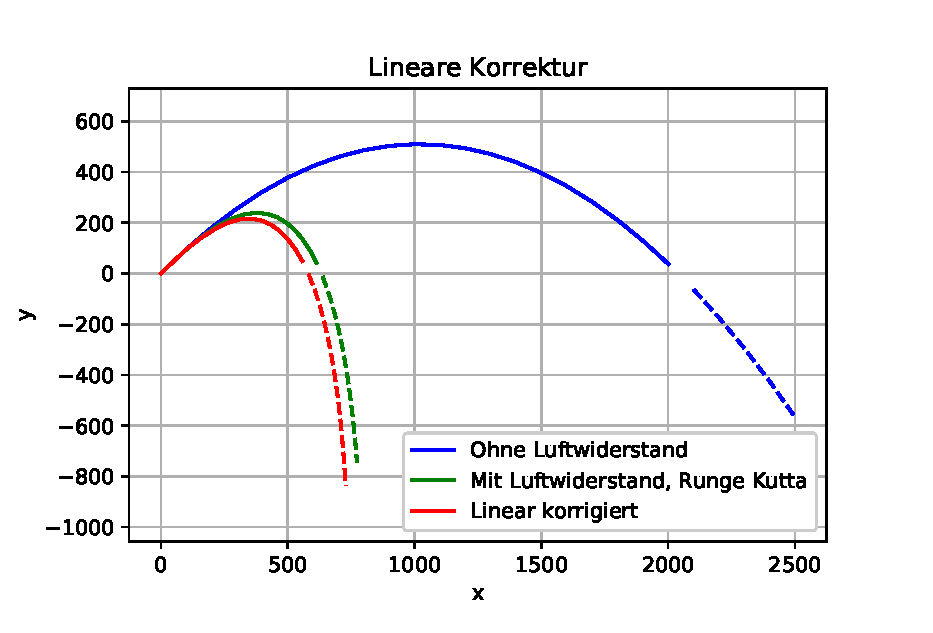
\includegraphics[scale=0.7]{papers/perturbation/bilder/perturbation_fig1.eps}
    \caption{Linearer Korrekturterm}
	\label{naive_linear_term}
\end{figure}


Anstelle des linearen Ansatzes könnte man auch einen quadratischen Ansatz nutzen.
Dies ergibt anstelle von \eqref{eq:x_linear}:
\begin{equation}
\begin{aligned}
x(t)
&=
x_0 + t \cdot (v_{0_x} + \phi_{x_1}t + \phi_{x_2}t^2)
&
&= x_0 + v_{0_x}t + \phi_{x_1}t^2 + \phi_{x_2}t^3\\
y(t)
&=
y_0 + t \cdot (v_{0_y} + \phi_{y_1}t + \phi_{y_2}t^2) - \frac{1}{2}gt^2
&
&= y_0 + v_{0_y}t + \phi_{y_1}t^2 + \phi_{y_2}t^3 - \frac{1}{2}gt^2.
\end{aligned}
\end{equation}


Damit haben wir noch bessere Resultate erhalten.
Diese sind in Abbildung \ref{naive_quadratic_term} ersichtlich.
Von Auge ist bereits kein Unterschied der beiden Flugbahnen mehr erkennbar.
\begin{figure}
    \centering
    \includegraphics[scale = 0.7]{papers/perturbation/bilder/perturbation_fig2.eps}
    \caption{Quadratischer Korrekturterm}
	\label{naive_quadratic_term}
\end{figure}

\section{Verbesserte Lösung
\label{perturbation:section:verbesserte_loesung}}
\rhead{Verbesserte Lösung}

Man erhält bessere Resultate, wenn man statt nur die Anfangswerte $\vec{v}_0 = (v_{0x}, v_{0y})$ auch $\vec{r}_0 = (r_{0x}, r_{0y})$ variabel gestaltet.
Zudem kann man anstelle von $t$ nur die Differenz $\Delta t$ seit dem letzten Update von der Bodenstation betrachten.

Wiederum ist das Ziel, dass der Flugkörper mit den einfachen Formeln \eqref{eq:x_simple} eine möglichst gute Approximation auf einfache Art und Weise berechnen kann,
indem er die Anfangswerte $\vec{r}_0$ und $\vec{v}_0$ im Laufe der Zeit gemäss Weisungen der Bodenstation anpasst.

In einem ersten Schritt verlangen wir von der Bodenstation, welche $\vec{r}$, aber auch $\vec{v}$ mit dem Runge-Kutta-Verfahren berechnen kann,
eben diese Werte um so eine Approximation mit den simplen Formeln \eqref{eq:x_simple} tätigen zu können.
Es ergeben sich folgende Formeln:

\begin{equation}
\begin{aligned}
r_x(t + \Delta t) &= r_{0x} + v_{0x}\Delta t\\
r_y(t + \Delta t) &= r_{0y} + v_{0y}\Delta t - \frac{1}{2}g\Delta t^2.
\end{aligned}
\end{equation}
Verlangt man von der Bodenstation jede Sekunde neue Werte für die Elemente $r_{0x}, r_{0y}, v_{0x}$ und $v_{0y}$ gibt dies eine Genauigkeit von 2 Stellen.
In Abbildung \ref{error} ist der Fehler ersichtlich.
Dieser ist als euklidische Distanz zur effektiven Position dargestellt.

\begin{figure}
    \centering
    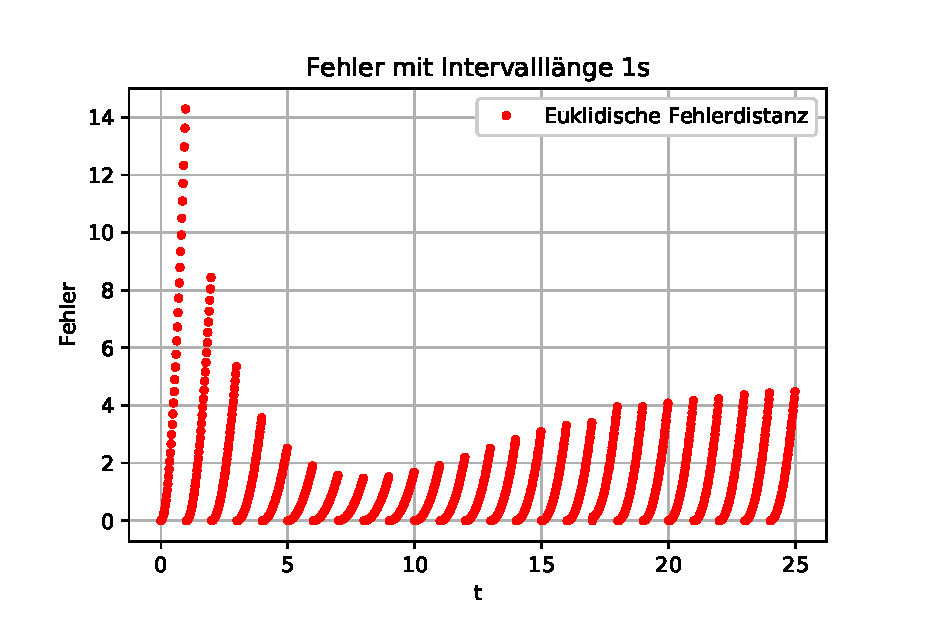
\includegraphics[scale = 0.7]{papers/perturbation/bilder/perturbation_fig3.eps}
    \caption{Fehler als euklidische Distanz}
	\label{error}
\end{figure}
\section{Möglichkeiten zur Genauigkeitssteigerung
\label{perturbation:section:weitereverbesserungen}}
\rhead{Weitere Verbesserungen}
In diesem Abschnitt diskutieren wir Verbesserungsmöglichkeiten, um den Fehler weiter zu minimieren. 
Abbildung \ref{error} zeigt, dass der Fehler stark von der Intervalllänge abhängt. 
Eine Reduktion der Intervallänge beschreiben wir im nächsten Abschnitt. Weiter lassen sich mit Hilfe der Störungstheorie höherer Ordnung genauere Resultate erzielen.

\subsection{Reduktion der Intervalllänge}
In Abbildung \ref{error} ist der Fehler für die Intervalllänge von einer Sekunde ersichtlich. 
Wie man erkennen kann, nimmt dieser innerhalb wenigen Millisekunden stark zu. 
Dies ist vor allem unserem Beispiel geschuldet, da die Störung (in unserem Beispiel der Luftwiderstand) kurzfristig eine grosse Auswirkung auf das Resultat hat. 
Bei Berechnungen von z.B. Satellitenbahnen wäre dies anders, da Störungen, wie die Gravitation von Planeten, viel kleiner sind und die Abweichungen erst bei längeren Intervalldauern auftreten.

Für unser Beispiel haben wir in einem ersten Schritt die Intervallänge halbiert und sind auf die Resultate in Abbildung \ref{errorShortInterval} gekommen. 
Wie ersichtlich ist, ist der Fehler um ca. Faktor 4 kleiner. 
Wir erhalten somit weitere 2 Bit Genauigkeitsgewinn. 
Weiter ist zum Zeitpunkt $t=17s$ eine kleine numerische Instabilität beobachtbar.

\begin{figure}
    \centering
    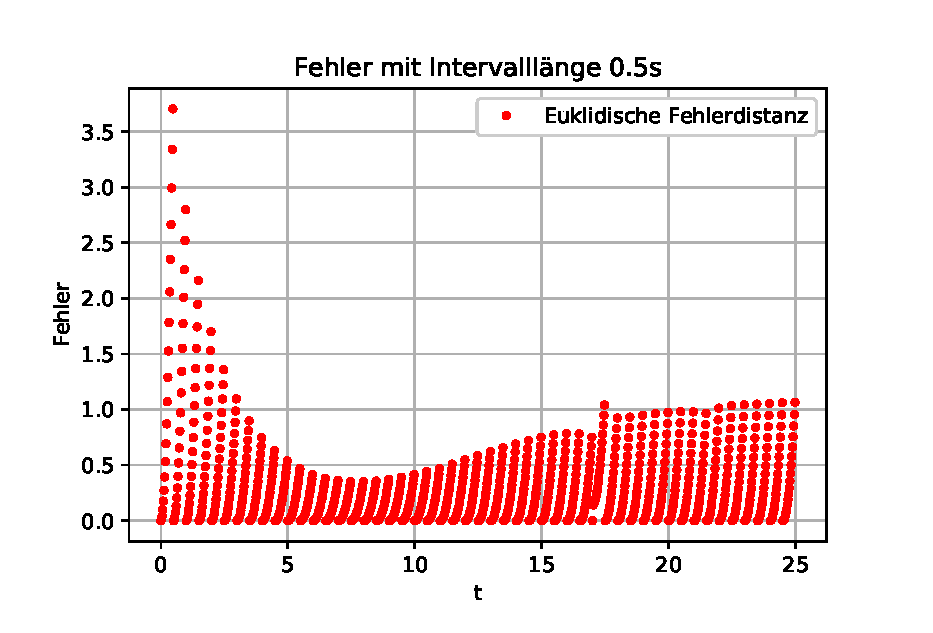
\includegraphics[scale=0.7]{papers/perturbation/bilder/perturbation_fig4.eps}
    \caption{Fehler bei halbierter Intervalldauer}
	\label{errorShortInterval}
\end{figure}

In einem zweiten Schritt haben wir die Intervallänge nochmals auf die Länge $\Delta t = 0.25$ halbiert. 
Dies ist in Abbildung \ref{errorShortInterval2} ersichtlich. 
Wir erhalten wieder einen Genaugikeitsgewinn um den Faktor 4 bzw. 2 Bit. 
Dies lässt sich leider jedoch nicht weiter beliebig fortsetzen. 
Die Rechenlast des Satelliten bleibt konstant und ist nicht von der Intervalllänge abhängig. 
Der Aufwand für die Bodenstation nimmt jedoch zu. 
Da die numerischen Berechnungen für aufwänderige Formeln (wie Satellitenbahnen) oft ein wenig dauern und gegebenfalls viel Rechenleistung benötigen, sind diese nicht günstig und können nicht beliebig oft ausgeführt werden.

\begin{figure}
    \centering
    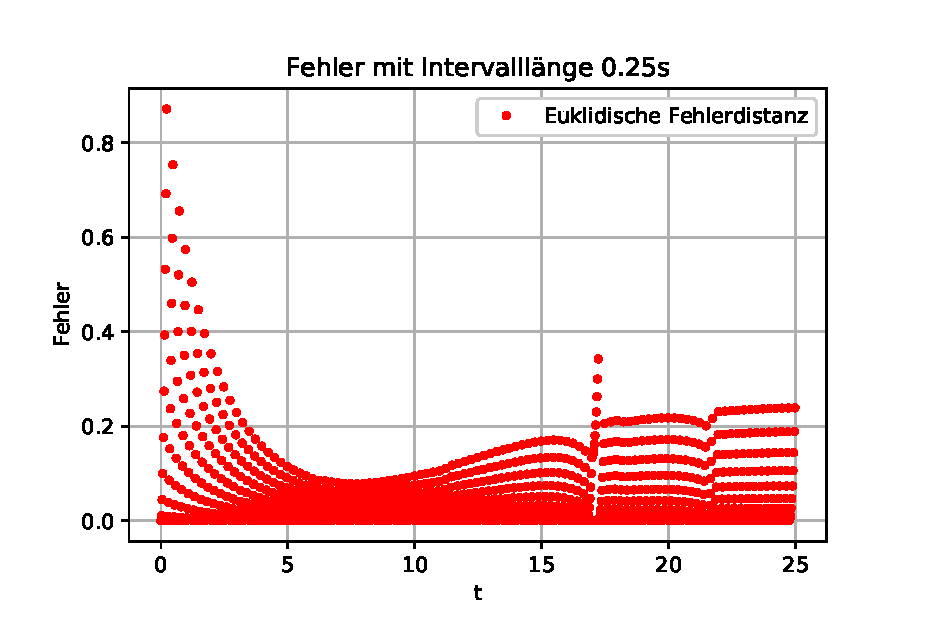
\includegraphics[scale=0.7]{papers/perturbation/bilder/perturbation_fig5.eps}
    \caption{Fehler mit einem Viertel der Intervalldauer}
	\label{errorShortInterval2}
\end{figure}

\subsection{Erhöhung der Ordnung}
Eine andere Möglichkeit zur Steigerung der Genauigkeit eröffnet sich dadurch, dass man anstelle $x_0, y_0, v_{0x}$ und $v_{0y}$, was an sich Polynome nullter Ordnung sind, Polynome höherer Ordnung ansetzt. Wir schauen uns ein Beispiel erster Ordnung an. Wir ändern nun die Anfangsbedingungen folgendermassen. Um die Notation klar zu halten, werden wir nicht länger $x_0$ und $y_0$ verwenden, sondern vom Ortsvektor $\vec{r_0}$ sprechen.

\begin{equation}
\label{eq:ordnung1_linear_ansatz}
\begin{aligned}
x_0 \longrightarrow & \textcolor{red}{r_{x0} +   r_{x1}  \cdot \Delta t}\\
y_0 \longrightarrow & \textcolor{red}{r_{y0} +   r_{y1}  \cdot \Delta t}\\
v_x \longrightarrow & \textcolor{blue}{v_{x0} + v_{x1}  \cdot \Delta t}\\
v_y \longrightarrow & \textcolor{blue}{v_{y0} + v_{y1}  \cdot \Delta t}\\
\end{aligned}
\end{equation}

Betrachten wir nun ein bestimmtes Intervall, etwa $t \in [5,6)$. Innerhalb dieses Intervalls arbeiten wir mit $t=5$, $\Delta t \in [0,1)$. 
t wird also fixiert und $\Delta t$ ist unsere neue Variable. 
So gilt nach Einsetzen in Gleichungen \eqref{eq:x_simple} 

%todo die zteilenabstände brauchts nicht, ist nur für mich zum fehler vermeiden (zur übersicht)
%kansnt alles wegmachen ;) schaut nmämlich ewtas komisch aus im pdf xD

\begin{equation}\label{eq:ordnung1_linear_r}\begin{aligned}
r_x(t + \Delta t) =& 
\textcolor{red}{(r_{x_0} +   r_{x_1}  \cdot \Delta t)} +
\textcolor{blue}{(v_{x_0} + v_{x_1}  \cdot \Delta t)} \cdot \Delta t \\
r_y(t + \Delta t) =& 
\textcolor{red}{(r_{y_0} +   r_{y_1} \cdot \Delta t)} +
\textcolor{blue}{(v_{y_0} + v_{y_1} \cdot \Delta t)} \cdot \Delta t -
\frac{1}{2}g \Delta t^2
\end{aligned}
\end{equation}

Um das Problem lösen zu können, werden wir auch eine exklusive Betrachtung der Geschwindigkeit durchführen. Indem man Gleichung \ref{eq:x_simple} nach $t$ ableitet und anschliessend unseren Ansatz für die Anfangsbedingungen einsetzt, erhält man

\begin{equation}\label{eq:ordnung1_linear_v}\begin{aligned}
v_x(t + \Delta t) =& 
\textcolor{blue}{(v_{x_0} + v_{x_1}  \cdot \Delta t)} \\
v_y(t+ \Delta t) =& 
\textcolor{blue}{(v_{y_0} + v_{y_1} \cdot \Delta t)} -
g \Delta t
\end{aligned}\end{equation}

\subsubsection{Lösung des Problems mit linearer Interpolation}\label{section:perturbation_ordnung1_linear}

In obigen Gleichungen sind die 8 Unbekannten $r_{x0}, r_{x1}, r_{y0}, r_{y1}, v_{x0}, v_{x1}, v_{y0}$ und $v_{y1}$ zu bestimmen. Zwar haben wir mit Gleichungen \ref{eq:ordnung1_linear_r} und \ref{eq:ordnung1_linear_v} nur vier Gleichungen, indem wir aber $\Delta t$ variieren, können wir die Anzahl Gleichungen beliebig erhöhen. Das Gleichungssystem ist somit lösbar. Wir machen uns hierbei zu Nutze, dass die Bodenstation mit dem Runge-Kutta Verfahren $\vec{r}(t + \Delta t)$ und $\vec{v}(t + \Delta t)$ liefern kann. Dies sind also bekannte Werte, unabhängig davon, wie $\Delta t$ gesetzt wird.\\

Indem wir $\Delta t = 0$ setzen, erhalten wir auf relativ einfache Art und Weise all jene Unbekannte, die mit einer $0$ indiziert sind. Die Lösung ergibt sich direkt aus obigen Gleichungen. Wir Nutzen hierbei Gleichung \eqref{eq:ordnung1_linear_r} zur Bestimmung von $\vec{r_0}$, und Gleichung \eqref{eq:ordnung1_linear_v} zur Bestimmung von $\vec{v_0}$.

\begin{equation}
\label{eq:ordnung1_linear_solutionPart1}
\begin{aligned}
r_{x0} =& r_x(t) \\
r_{y0} =& r_y(t) \\
v_{x0} =& v_x(t) \\
v_{y0} =& v_y(t) \\
\end{aligned}
\end{equation}

Um $v_{x1}$ und $v_{y1}$ zu bestimmen, können wir nun weiterhin Gleichung \ref{eq:ordnung1_linear_v} verwenden, müssen aber das $\Delta t$ alternieren. Mit einer linearen Interpolation bietet sich $\Delta t = 1s$ an. Man könnte aber auch z.B. die halbe Intervalldauer $\Delta t = 0.5s$ wählen. Mit einer einfachen Umformung ergibt sich:

\begin{equation}
\label{eq:ordnung1_linear_solutionPart2}
\begin{aligned}
v_{x1} =& \frac{v_x(t + \Delta t) - v_{x0}}{\Delta t} \\
v_{y1} =& \frac{v_y(t + \Delta t) - v_{y0} + g \cdot t}{\Delta t}
\end{aligned}
\end{equation}

Wie zu erkennen ist, machen wir bereits Gebrauch von den zuvor bestimmten Unbekannten. Zu guter letzt können mit Gleichung \ref{eq:ordnung1_linear_r} die zwei verbleibenden Unbekannten bestimmt werden:

\begin{equation}
\label{eq:ordnung1_linear_solutionPart3}
\begin{aligned}
r_{x_1} =& \frac{r_x(t + \Delta t) - r_{x0} - \Delta t \cdot(v_{x0} + v_{x1}  \cdot \Delta t)}{\Delta t} \\
r_{y_1} =& \frac{r_y(t + \Delta t) - r_{y0} - \Delta t \cdot(v_{y0} + v_{y1}  \cdot \Delta t) + 0.5gt^2}{\Delta t}
\end{aligned}
\end{equation}


Somit sind nun alle Unbekannten bestimmt und Gleichung \eqref{eq:ordnung1_linear_r} kann zur Bestimmung des Ortes herangezogen werden. Berechnen wir die Position schrittweise für die Intervalle $\{[0,1), [1, 2), \dots\}$ ergibt sich die euklidische Fehlerdistanz in Bild \ref{fig:ordnung1_linear_error_A}.

Anstelle der Interpolation an den Stützstellen $\Delta t = 0$ und $\Delta t = 1$ liessen sich, wie bereits erwähnt, auch die Stützstellen $\Delta t = 0$ und $\Delta t = 0.5s$ nutzen. Dies führt zu der Fehlerverteilung gemäss Bild \ref{fig:ordnung1_linear_error_B}.

In beiden Grafiken ist schön zu erkennen, wie der Fehler jeweils bei einer Stützstelle auf $0$ sinkt, zwischen den Stützstellen aber einen Anstieg verzeichnet. Es ist auch gut zu erkennen, dass die Wahl der Stützstellen jeweils am Anfang und am Ende erfolgen sollte, um einen maximalen Bereich des Intervalls abzudecken. 

Vergleichen wir den Fehler aus Grafik \ref{fig:ordnung1_linear_error_A} mit Polynomen nullter Ordnung in Grafik \ref{error} erkennen wir erneut eine Genauigkeitssteigerung um Faktor vier. Die Erhöhung der Ordnung um eins hat also den selben Effekt wie wie Halbierung der Intervalldauer.

Selbstverständlich könnte der Anwender auch beide Verfahren kombinieren. Der Fehler, stets als euklidische Distanz zum echten Standort dargestellt, mit Ordnung 1 und Intervalldauer $0.5s$ ist in Grafik \ref{fig:ordnung1_linear_error_C} abgebildet. Erneut ist der Fehler viermal kleiner geworden. Die Abweichung beträgt nun nur noch maximal $1m$.

\begin{figure}
	\centering
	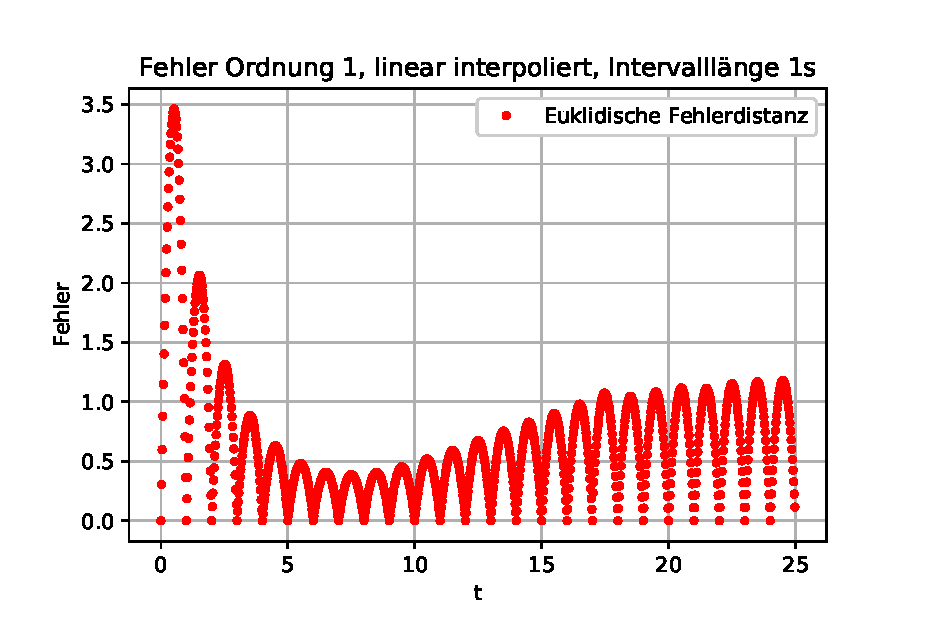
\includegraphics[scale=0.7]{papers/perturbation/bilder/perturbation_fig6.eps}
	\caption{Fehler bei Polynomen erster Ordnung}
	\label{fig:ordnung1_linear_error_A}
\end{figure}

\begin{figure}
	\centering
	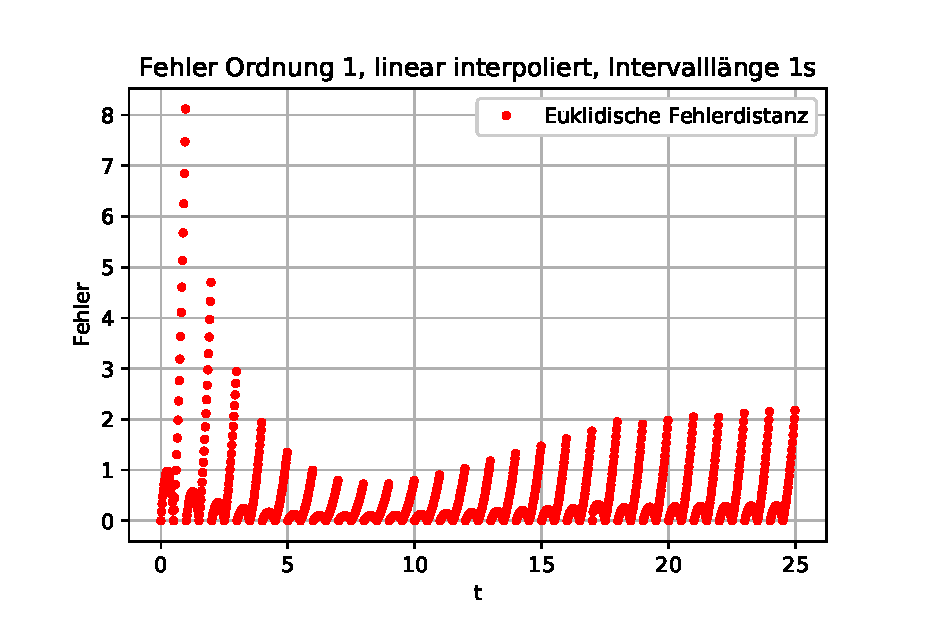
\includegraphics[scale=0.7]{papers/perturbation/bilder/perturbation_fig7.eps}
	\caption{Fehler bei Polynomen erster Ordnung mit variierten Stützstellen}
	\label{fig:ordnung1_linear_error_B}
\end{figure}

\begin{figure}
	\centering
	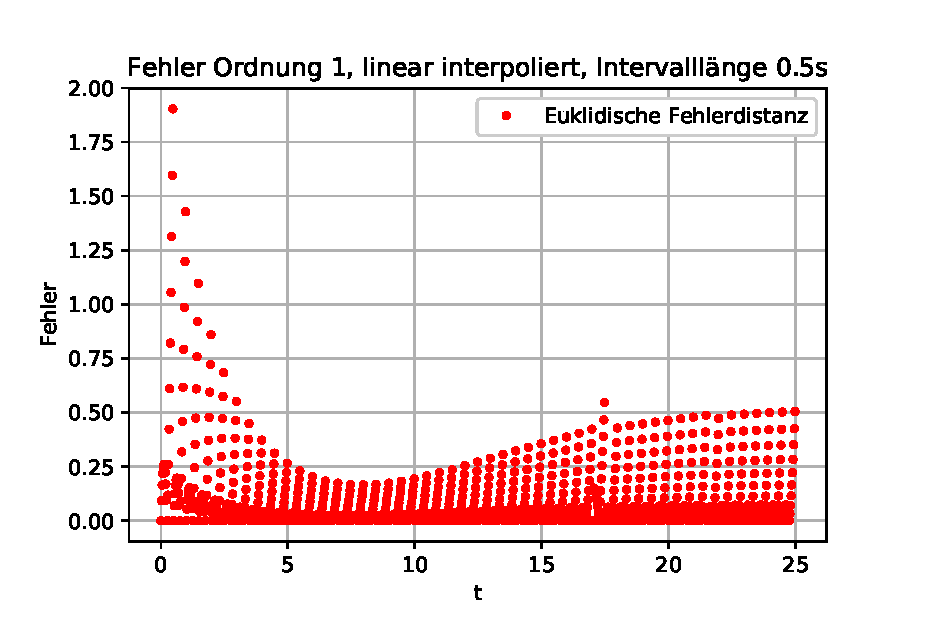
\includegraphics[scale=0.7]{papers/perturbation/bilder/perturbation_fig8.eps}
	\caption{Fehler bei Polynomen erster Ordnung mit halbierter Intervalldauer}
	\label{fig:ordnung1_linear_error_C}
\end{figure}

\subsubsection{Lösung des Problems mit Taylorreihen}
Anstelle von linearer Interpolation, kann man die Unbekannten $r_{x0}, r_{x1}, r_{y0}, \dots$ auch mit anderen Verfahren bestimmen. 
Wir können den Ansatz \eqref{eq:ordnung1_linear_ansatz} als Taylorentwicklungen interpretieren. 
Betrachten wir nur die Ortskoordinate und leiten wir diese nach $\Delta t$ ab, erhalten wir das folgende System. Um die Notation kurz zu halten, verwenden wir Vektornotation anstelle der Aufteilung nach $x$- und $y$-Komponenten.

\begin{equation}
\label{eq:ordnung1_taylor_ansatz}
\begin{aligned}
\vec{r} = & \vec{r_0} + \vec{r_1} \cdot \Delta t \\
\vec{\dot{r}} = & \vec{r_1} \\
\end{aligned}
\end{equation}

Die Unbekannte $\vec{r_0}$ ist erneut durch setzen von $\Delta t = 0$ sehr einfach zu erlangen, analog zu Kapitel \ref{section:perturbation_ordnung1_linear}. $\vec{r_1}$ kann ebenfalls ohne grossen Aufwand bestimmt werden, indem wir die Ableitung mit Hilfe der Bodenstation wie folgt annähern:
\[
\vec{\dot{r}}(t) \approx \frac{\vec{r}(t+\epsilon) - \vec{r}(t)}{\epsilon}
\]

Damit ist bereits eine Annäherung des Ortes möglich. Analog könnte man auch die Geschwindigkeit betrachten.

Beide Varianten, Interpolation und Taylorentwicklung, sind legitim. Die Interpolation ist am Anfang und Ende des Intervalles exakt, hat dafür aber in der Mitte einen relativ hohen Fehler. Die Taylorentwicklung ist vor allem zu Beginn des Intervalls exakt. Dies, da insbesondere bei höheren Ordnungen auch die Krümmung des Kurvenverlaufs berücksichtigt wird. Da sich allerdings alle Stützstellen am Anfang des Intervalles befinden, wird der Kurvenverlauf zum Ende des Intervalles hin immer ungenauer.

\section{Fazit}
Durch das Studium der Störungstheorie haben wir gesehen, dass auch komplexe Bahnverläufe mit begrenzter Rechenleistung sehr gut approximiert werden können.
Man benötigt allerdings eine Bodenstation, die fähig ist, exakte Werte an vorgegebenen Stützstellen zu berechnen.
Dies kann mit Hilfe numerischer Verfahren zur Lösung komplexer Differentialgleichungen erreicht werden, wie beispielsweise dem Runge-Kutta-Verfahren.
Es lassen sich somit Verfahren kreieren, sodass auch ein Satellit oder ein anderes Objekt mit begrenzter Rechenleistung die Bahn approximieren kann.
Dies, obwohl die Bahn von hunderten planetarischen Objekten gestört wird.
Es ist dabei möglich, die Genauigkeit nahezu beliebig zu erhöhen, indem man entweder die Bodenstation in kürzeren Intervallen um neue Werte bittet,
oder Polynome höherer Ordnung anstelle der Anfangswerte einsetzt.

\printbibliography[heading=subbibliography]
\end{refsection}
